\chapter{نتایج و پیشنهادات}
در این فصل ابتدا نتایج حاصل از پیاده‌سازی الگوریتم توضیح داده‌شده در فصل قبل را برای هر دو سناریو مورد بررسی قرار میدهیم و سپس به دو مورد از کارهایی که در آینده برای پیشبرد این تحقیق و کمک به سایر محققان قابل انجام است اشاره میکنیم.
\newpage
%%%%%%%%%%%%%%%%%%%%%%%%%%%%%%%%%%%%%%%%%%%
\section{نتایج}
در این بخش، سناریو را در 2 حالت بدون مانع و همراه با مانع شبیه‌سازی میکنیم. جهت اینکار، پارامترهای لازم در این شبیه‌سازی را مطابق مقادیر زیر قرار داده و برای \lr{M1} هایی که مضرب 10 هستند و برای هر \lr{M1} 10 بار شبیه‌سازی را اجرا کرده و مقادیر را درونیابی میکنیم تا به نمودارهای زیر برسیم.
مقادیر قرار داده‌شده در شبیه‌سازی به شرح زیر است:

	- تعداد المان‌های آنتن: 20 = \lr{N}
	
	- تعداد المان‌های سطح هوشمند دوم: 20 = \lr{M2}
	
	- وزن نرخ هر کاربر: 1
	
	- مجموع توان دو کاربر: 10 میلی وات
	
	- انحراف از معیار نویز: \lr{0.0001}
	
	- ضریب افت توان مسیر دید مستقیم: \lr{2.5}
	
	- ضریب افت توان مسیر بین آنتن و سطوح هوشمند یا سطوح هوشمند و کاربر: 2
	
	- ضریب افت توان مسیر بین سطوح هوشمند: \lr{1.8}
	
	- فاصله‌ کاربر 1 تا آنتن: 50 متر
	
	- فاصله‌ کاربر 2 تا آنتن: 60 متر
	
	- فاصله سطح هوشمند 1 تا آنتن: 20 متر
	
	- فاصله سطح هوشمند 2 تا آنتن: 30 متر
	
	- فاصله کاربر 1 تا سطح هوشمند 1: 50 متر

	- فاصله کاربر 1 تا سطح هوشمند 2: 30 متر
	
	- فاصله کاربر 2 تا سطح هوشمند 1: 40 متر
	
	- فاصله کاربر 2 تا سطح هوشمند 2: 20 متر
	
	- فاصله بین سطوح هوشمند: 40 متر
	
	- طول گام الگوریتم گرادیان نزولی: \lr{0.1}
	
%%%%%%%%%%%%%%%%%%%%%%%%%%%%%%%%%%%%%%%%%%%
\newpage
\subsection{نتایج و تحلیل بهینه‌سازی بدون مانع}
طبق شرایط بالا و در حالت بدون مانع، شبیه‌سازی را اجرا کرده و نمودارهای زیر برای نرخ کاربر 1، کاربر 2 و مجموع نرخ هر دو کاربر رسم‌ شده است:

\begin{figure}[!h]
	\begin{minipage}{0.5\textwidth}
		\centering
		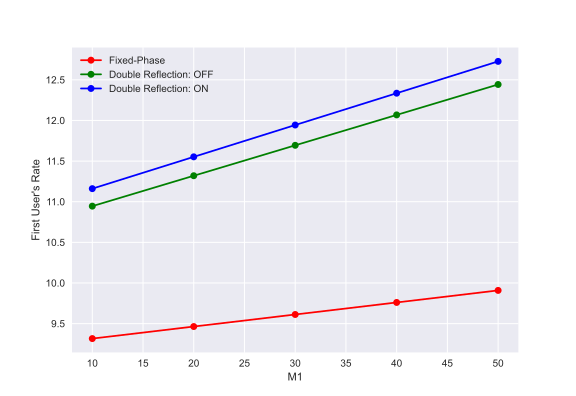
\includegraphics[scale=0.1]{No Blockage First User's Rate}
		\captionsetup{width=0.8\linewidth}
		\caption[
		نرخ کاربر اول در شرایط بدون مانع
		]{
			نرخ کاربر اول در شرایط بدون مانع
		}
%		\label{fig:Picture-2_06}
	\end{minipage}
	\hfill
	\begin{minipage}{0.5\textwidth}
		\centering
		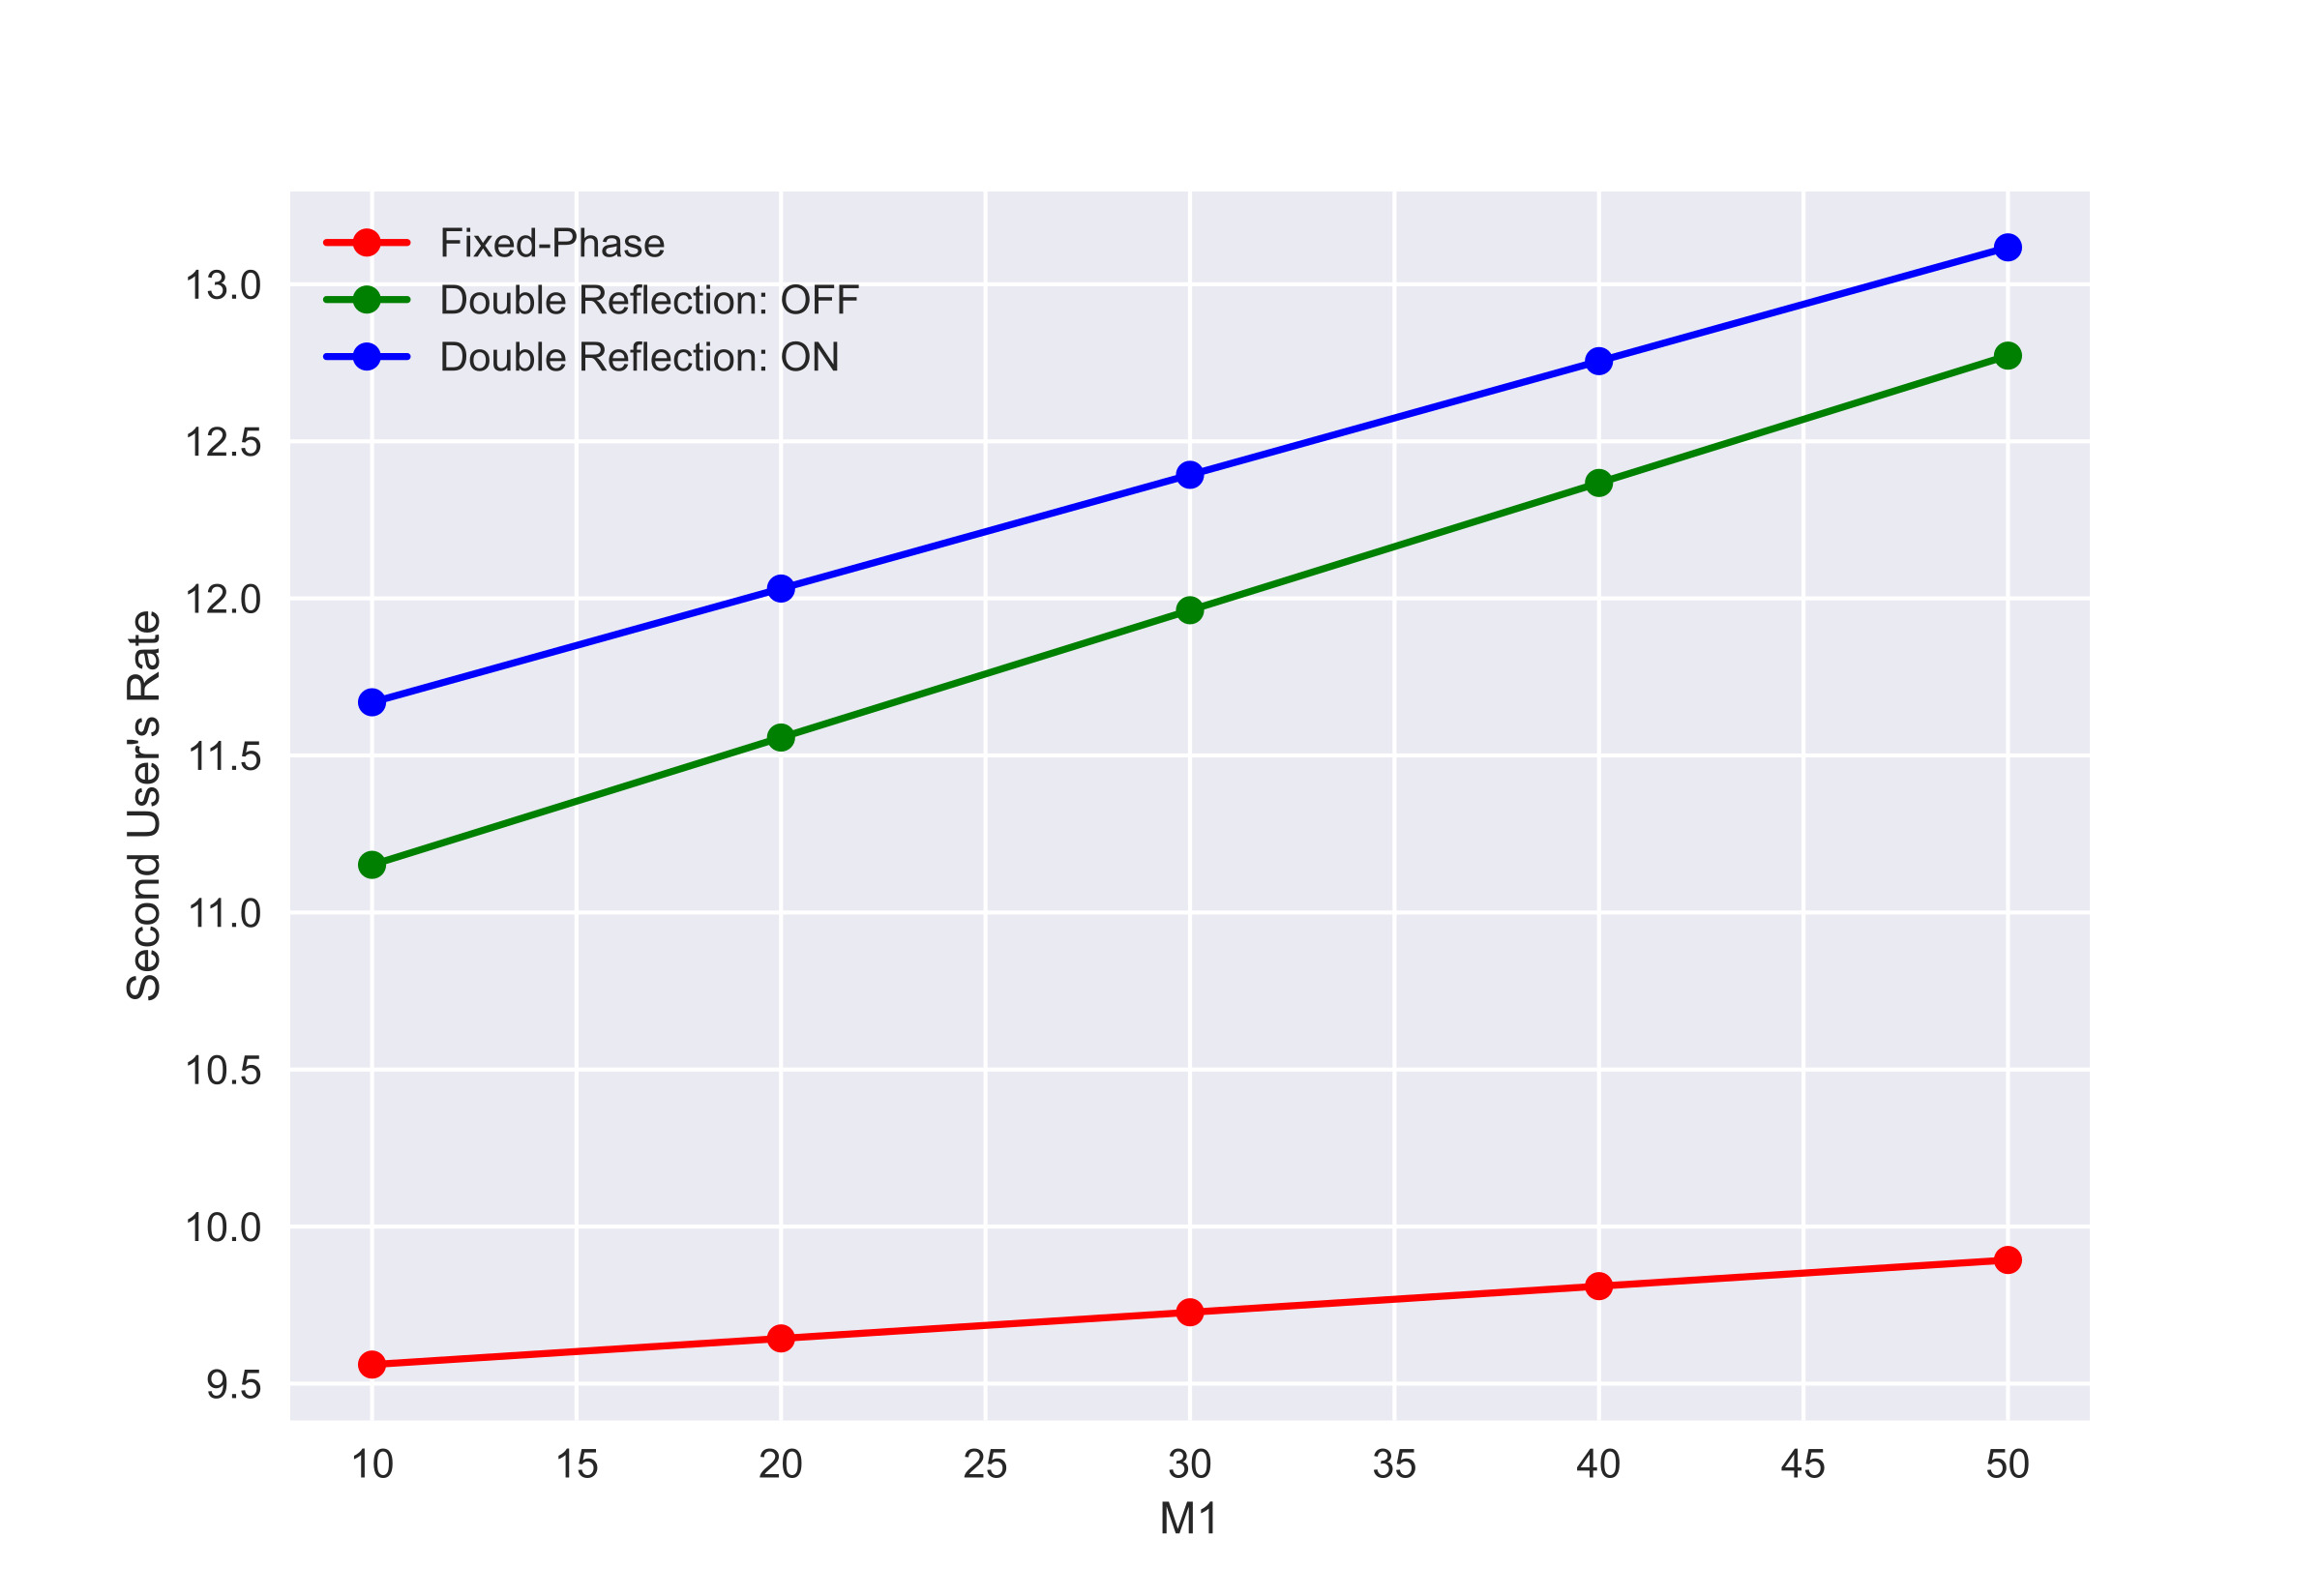
\includegraphics[scale=0.1]{No Blockage Second User's Rate}
		\captionsetup{width=0.8\linewidth}
		\caption[
		نرخ کاربر دوم در شرایط بدون مانع
		]{
		نرخ کاربر دوم در شرایط بدون مانع
		}
%		\label{fig:Picture-2_07}
	\end{minipage}
\end{figure}

\begin{figure}[!h]
	\centering
	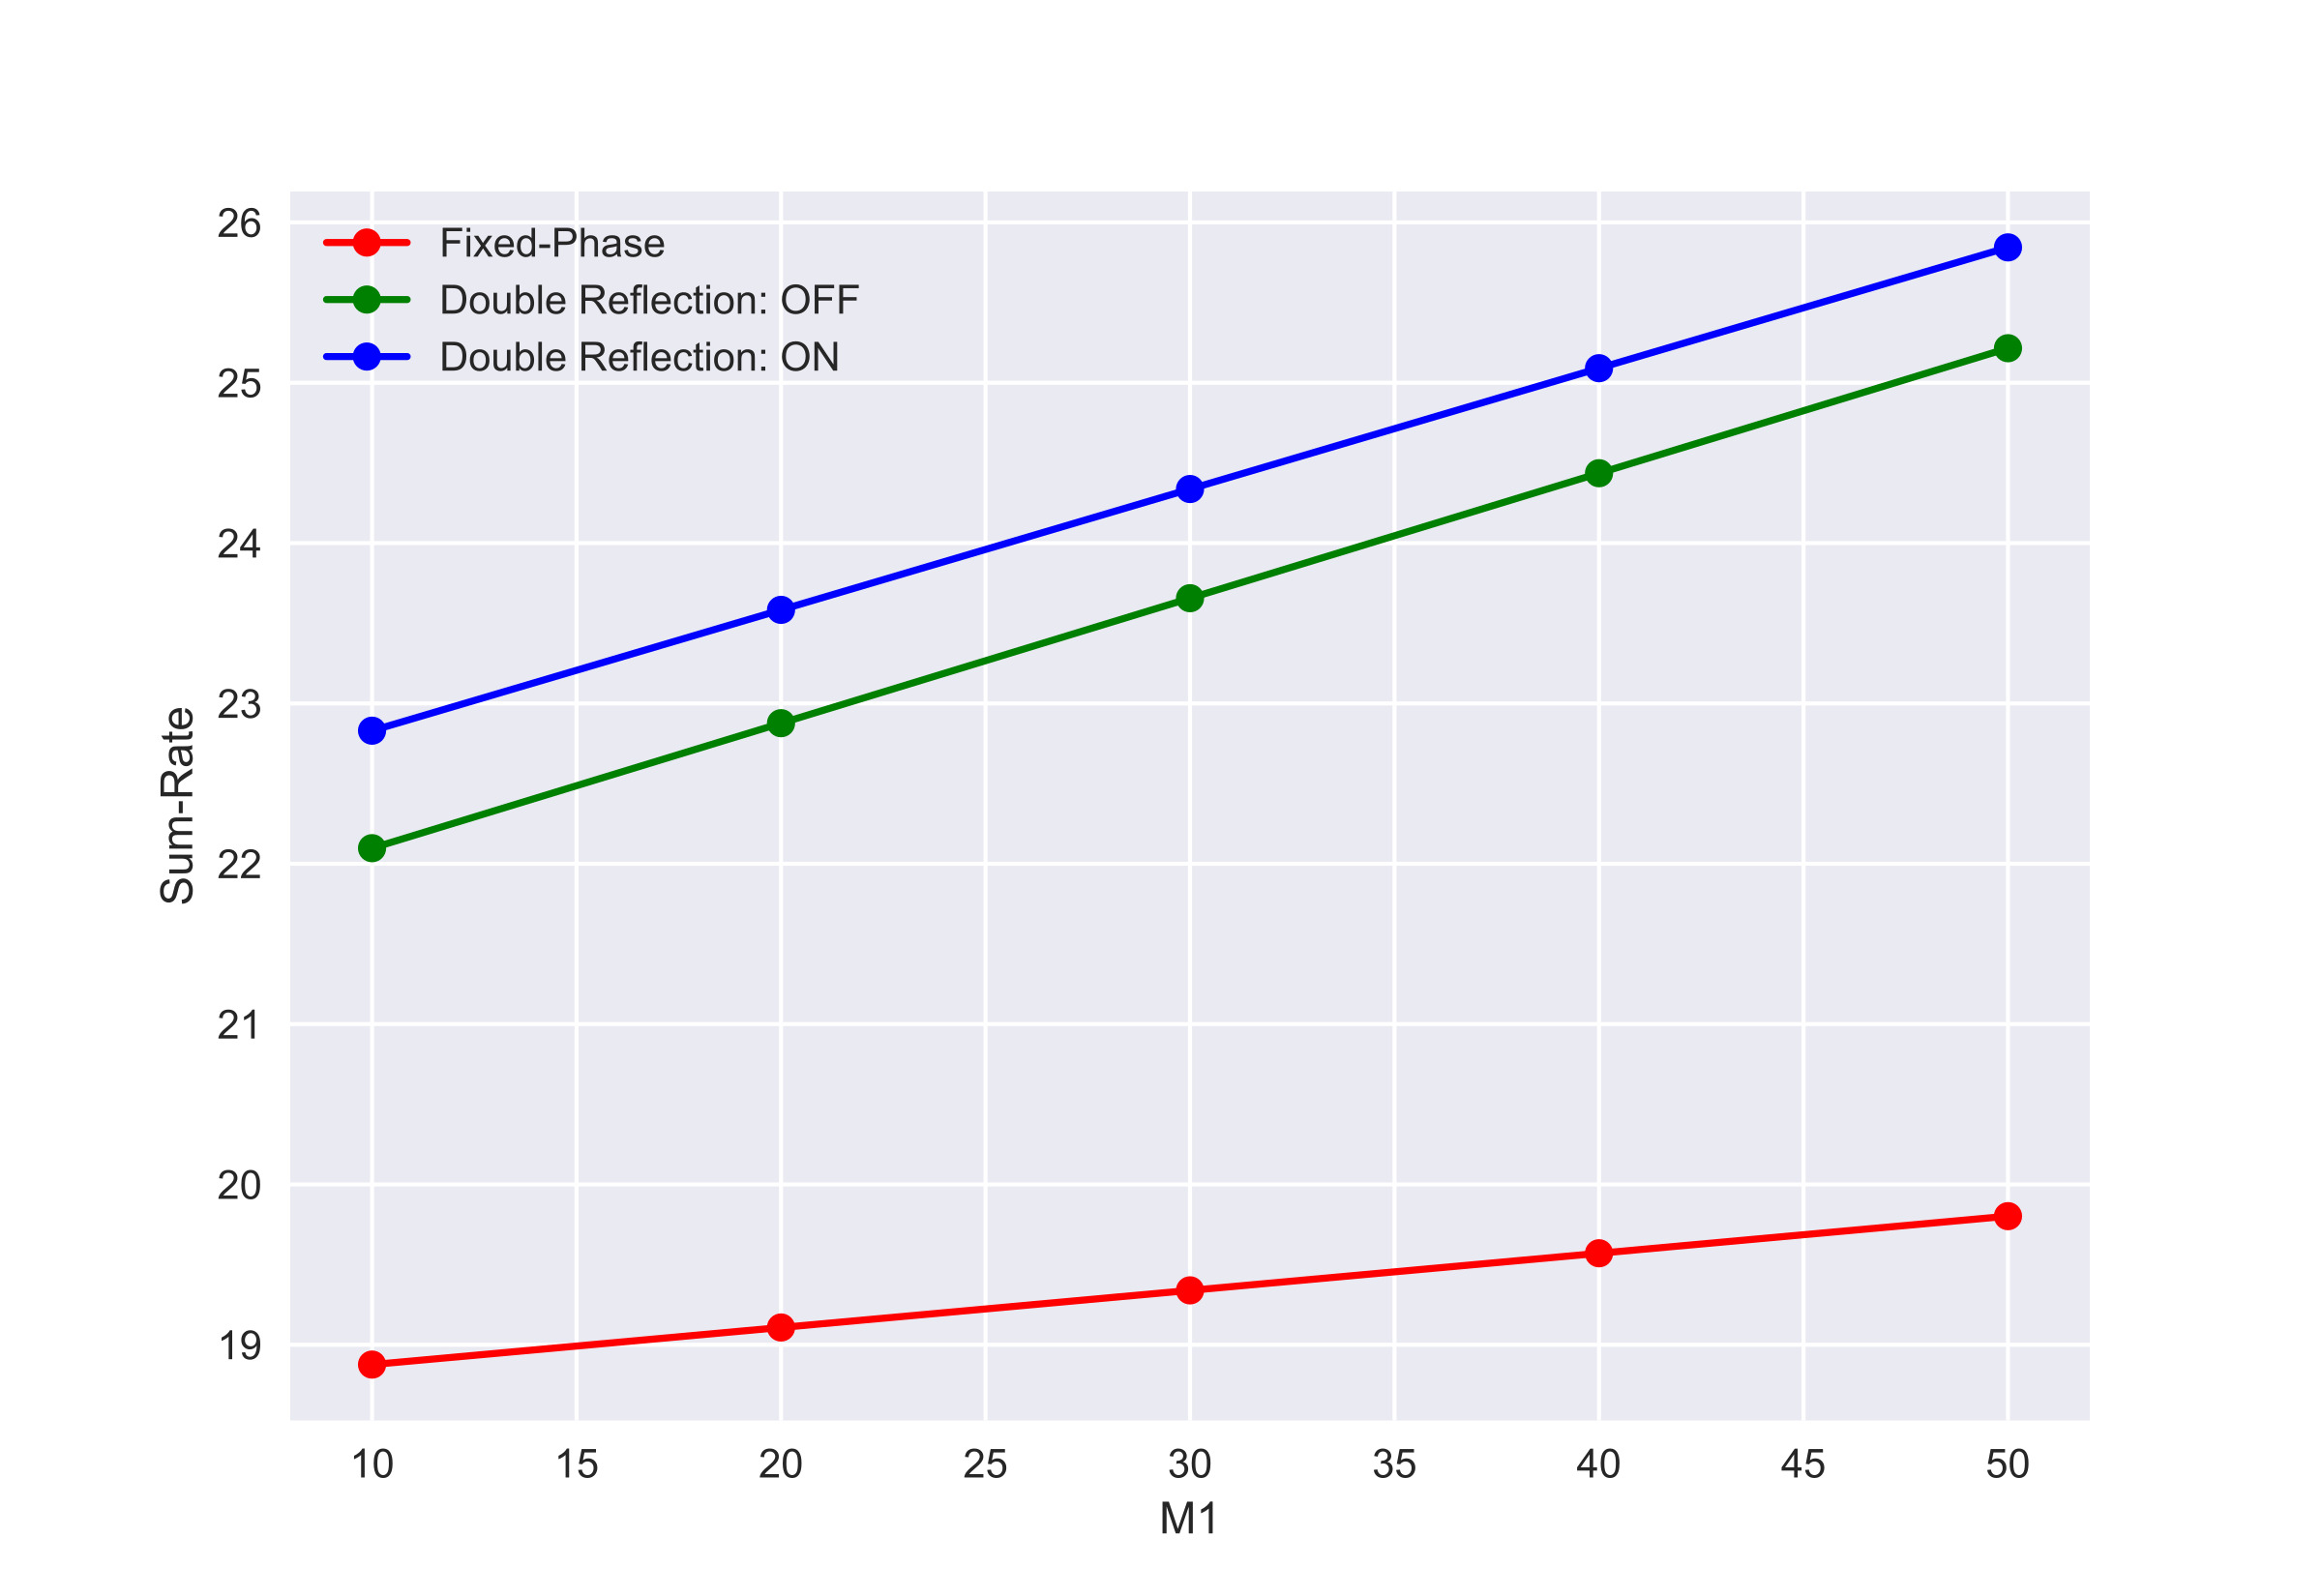
\includegraphics[scale=0.19]{No Blockage Sum-Rate}
	\caption[مجموع نرخ دو کاربر در شرایط بدون مانع]{
		مجموع نرخ دو کاربر در شرایط بدون مانع
	}
	%	\label{fig:fig-2_0}
\end{figure}

تحلیل: همانطور که مشاهده میشود در حالتی که سیگنال بازتابی بین سطوح در نظر گرفته شده‌است هر دو کاربر بهبودی را در سیگنال‌های دریافتی مشاهده میکنند اما نکته قابل توجه اینست که با در نظر گرفتن سیگنال بین سطوح باعث ایجاد پیچیدگی در بهینه‌سازی میشویم و زمان اجرا کندتر میشود و این موضوع میتواند سیستم را از حالت \lr{real time} خارج سازد پس باید هر شخص متناسب با سناریو خود بررسی کند که آیا این مقدار بهبود به اندازه پیچیدگی ایجاد شده ارزش دارد یا خیر؟
%%%%%%%%%%%%%%%%%%%%%%%%%%%%%%%%%%%%%%%%%%%
\newpage
\subsection{نتایج و تحلیل بهینه‌سازی با مانع}
طبق شرایط بالا و در حالت با مانع، شبیه‌سازی را اجرا کرده و نمودارهای زیر برای نرخ کاربر 1، کاربر 2 و مجموع نرخ هر دو کاربر رسم‌ شده ‌است:

\begin{figure}[!h]
	\begin{minipage}{0.5\textwidth}
		\centering
		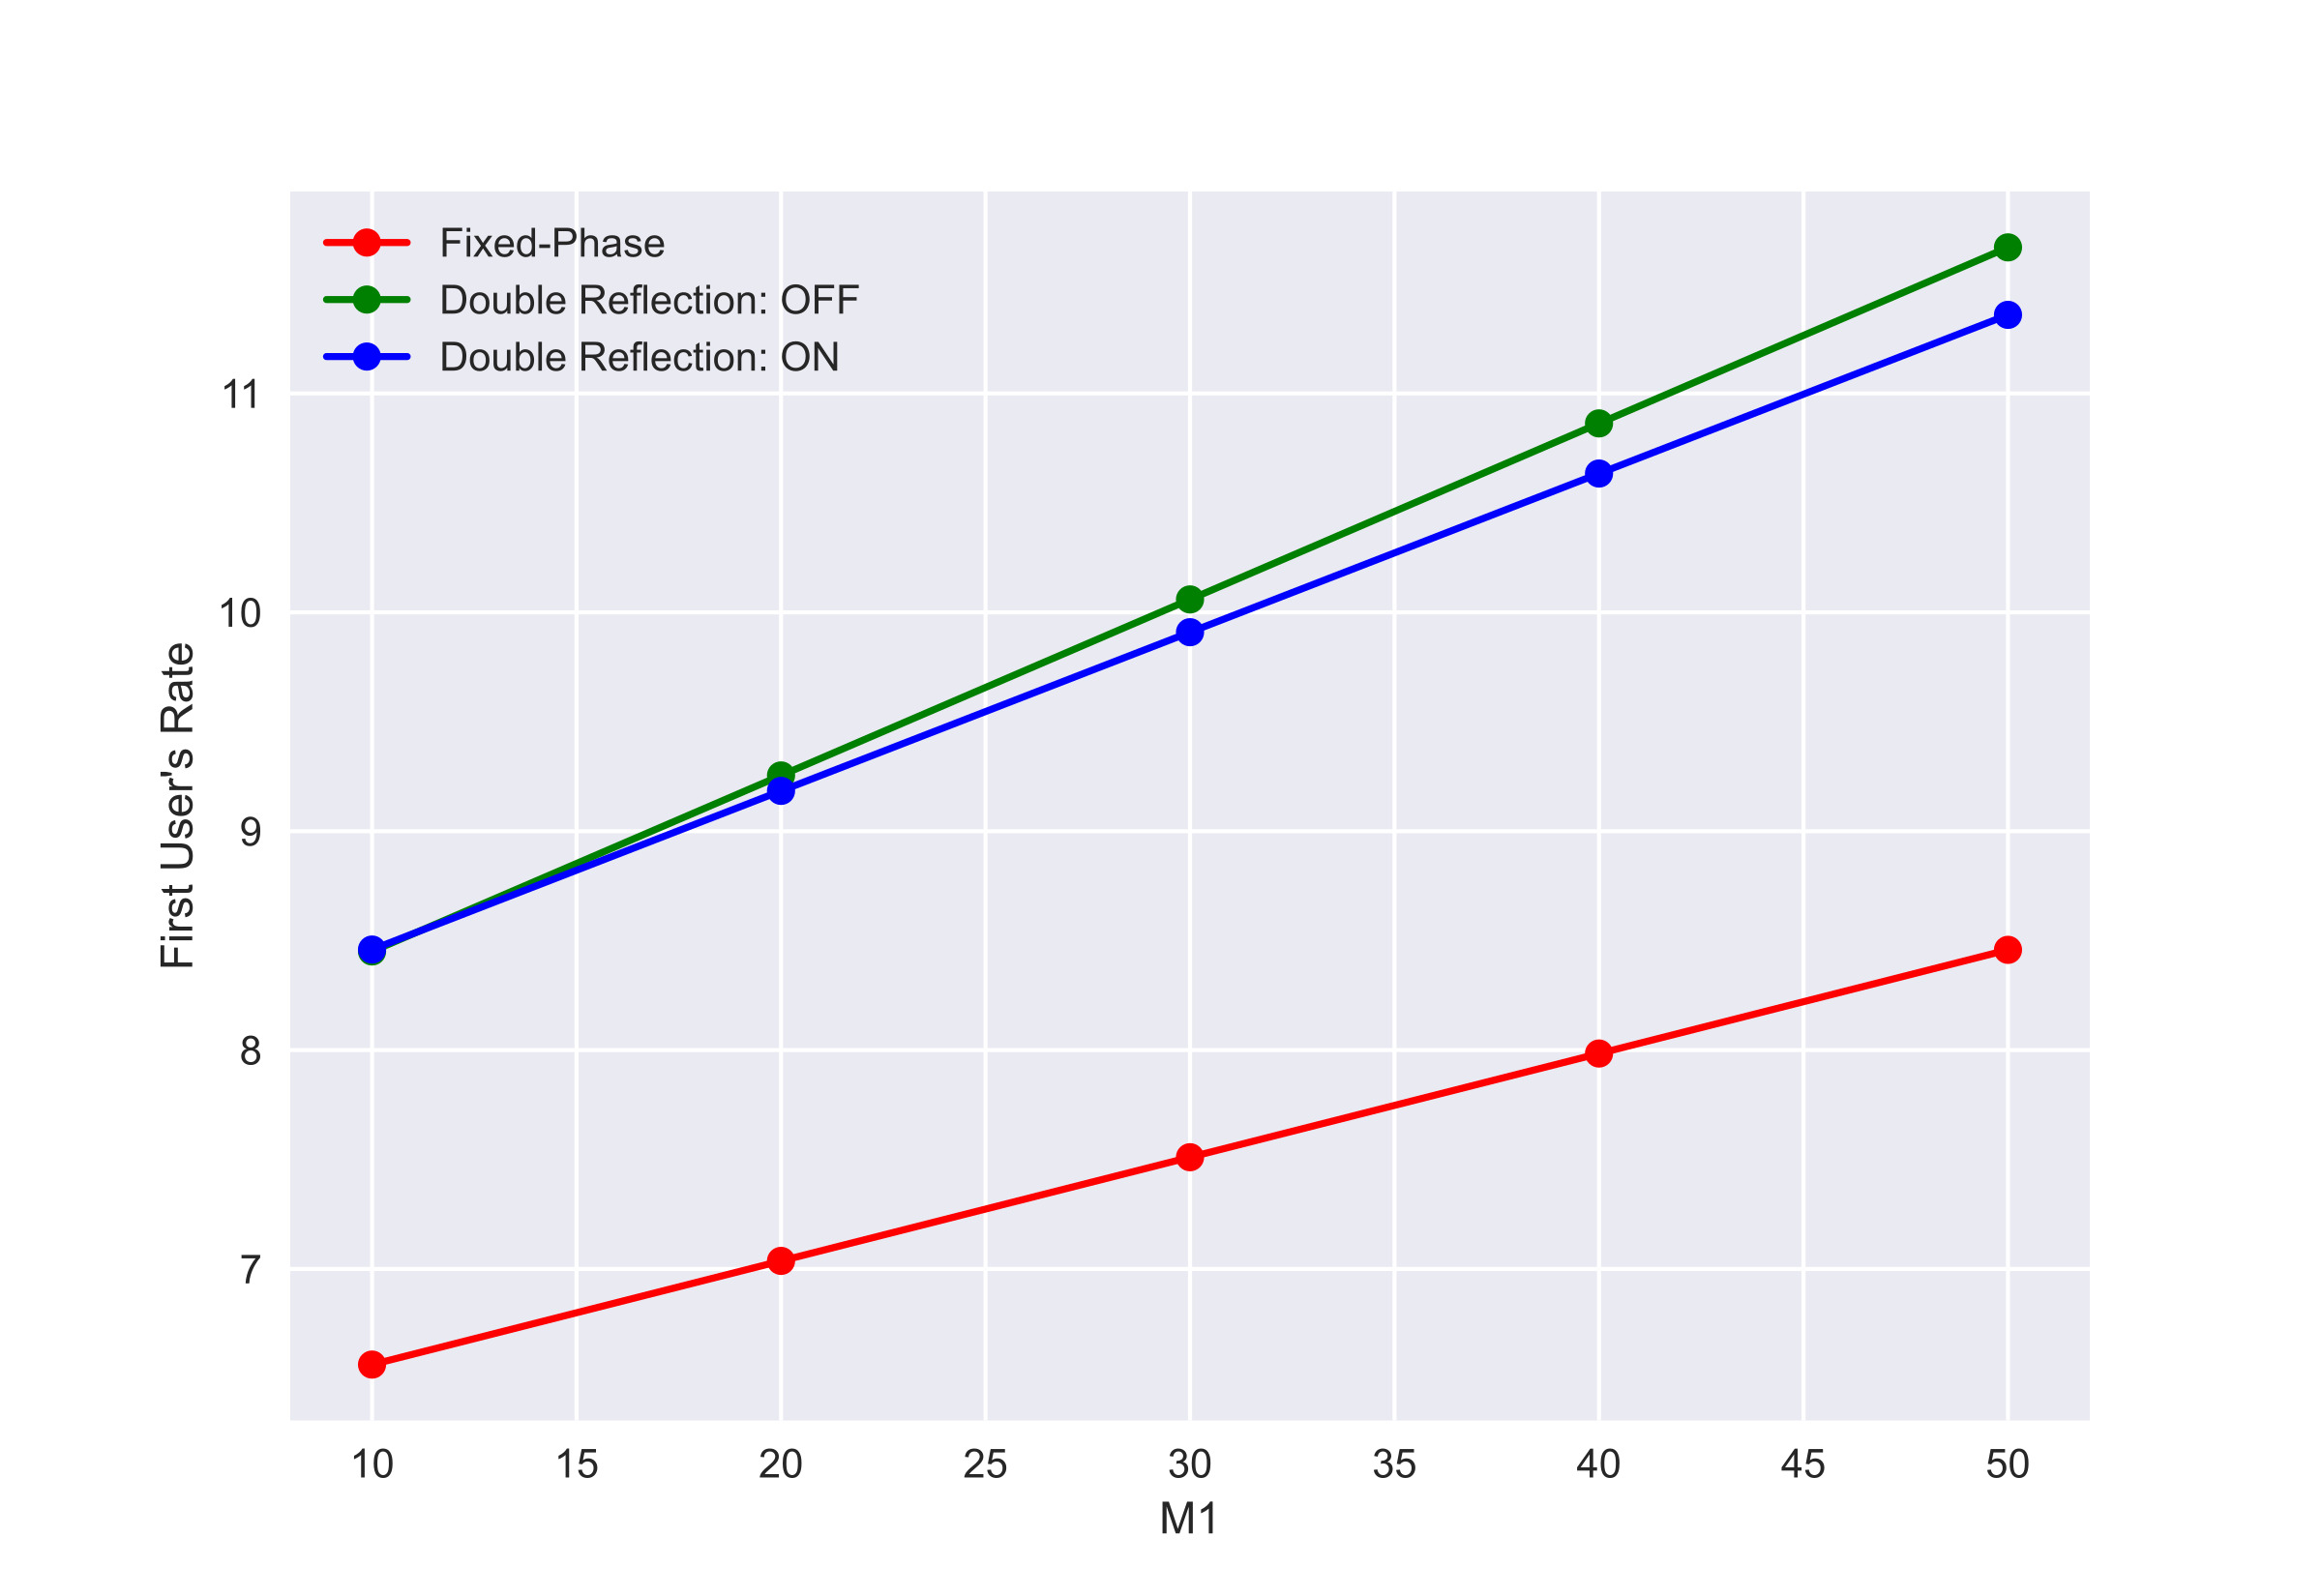
\includegraphics[scale=0.1]{With Blockage First User's Rate}
		\captionsetup{width=0.8\linewidth}
		\caption[
		نرخ کاربر اول در شرایط با مانع
		]{
		نرخ کاربر اول در شرایط با مانع
		}
%		\label{fig:Picture-2_006}
	\end{minipage}
	\hfill
	\begin{minipage}{0.5\textwidth}
		\centering
		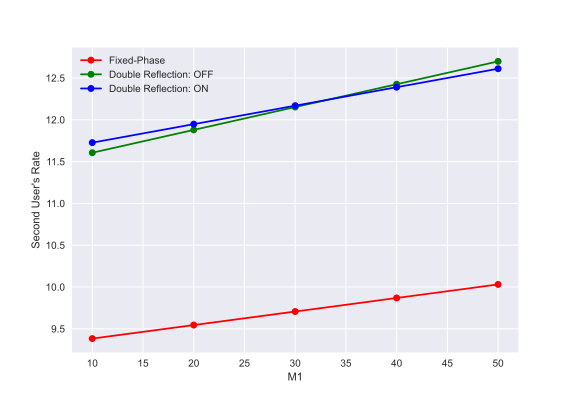
\includegraphics[scale=0.1]{With Blockage Second User's Rate}
		\captionsetup{width=0.8\linewidth}
		\caption[
		نرخ کاربر دوم در شرایط با مانع
		]{
			نرخ کاربر دوم در شرایط با مانع
		}
%		\label{fig:Picture-2_007}
	\end{minipage}
\end{figure}

\begin{figure}[!h]
	\centering
	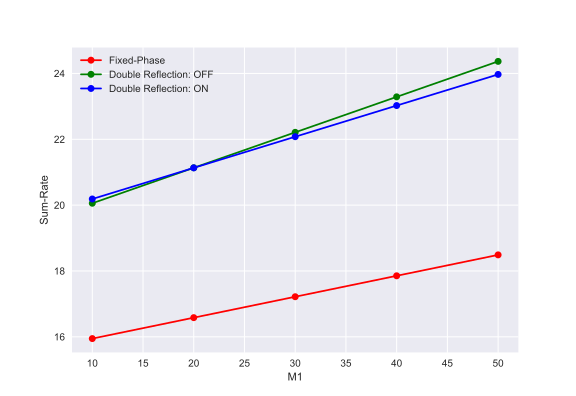
\includegraphics[scale=0.19]{With Blockage Sum-Rate}
	\caption[
	مجموع نرخ دو کاربر در شرایط با مانع
	]{
		مجموع نرخ دو کاربر در شرایط با مانع
	}
	%	\label{fig:fig-2_0}
\end{figure}

تحلیل: همانطور که مشاهده میشود در حالتی که سیگنال بازتابی بین سطوح در نظر گرفته شده‌است، هیچ‌یک از کاربرها بهبود خاصی را مشاهده نمیکنند و فقط با ایجاد پیچیدگی زمانی در مسئله، باعث کاهش سرعت همگرایی آن شده‌ایم. پس در این سناریو و سناریوهای مشابه استفاده از سیگنال بین سطوح توصیه نمیشود زیرا میتواند بدون هیچ بهبودی، باعث افزایش محاسبات و در نتیجه کاهش سرعت همگرایی شود.

\newpage
%%%%%%%%%%%%%%%%%%%%%%%%%%%%%%%%%%%%%%%%%%%
\section{پیشنهادات}

در این بخش به بررسی سه پیشنهاد(کارهای آینده) میپردازیم که میتواند توجه زیادی را به خود جلب کرده و مشکلات زیادی را حل کند:

\subsection{بازتاب مرتبه 3}

همانطور که دراین ستاریو بررسی شد، بازتاب بین سطوح هوشمند فقط تا بازتاب مرتبه 1 لحاظ شده است و در بخش نتایج مشاهده شد که این بازتاب، تاثیر چندانی بر روی بهینه شدن خروجی به نسبت پیچیدگی که به مسئله اضافه میکند، ندارد اما گاهی ناچار هستیم که این بازتاب را لحاظ کنیم. مثلا در هنگامی که دید مستقیم به فرستنده و یکی از دو سطوح هوشمند وجود ندارد، ناچار به لحاظ این بازتاب هستیم. 

اکنون یکی از مسائلی که مطرح میشود، این است که اگر 3 سطح هوشمند استفاده کنیم و دید مستقیم به دو سطح نداشته باشیم، آیا از نظر  نرخ دریافتی کاربر، بهینه است که از سیگنال بازتابی مرتبه 2 استفاده کنیم تا اطلاعات را به کاربر برسانیم؟

این یکی از سوالاتی است که میتواند در آینده و به کمک سایر محققان جواب داده شود. 

\subsection{ساخت فریم‌ورک برای بهینه‌سازی سطوح هوشمند}
یکی از چالش‌های اصلی که در برنامه‌نویسی این پروژه برای بهینه‌سازی ضرایب فاز وجود داشت، نبود هیچ فریم‌ورک یا همان چارچوب برنامه‌نویسی خاصی برای حل این مسائل است. ابتدا مجبور بودیم به دنبال الگوریتم بهینه بگردیم و سپس این الگوریتم را پیاده‌سازی نماییم و این امکان وجود داشت که الگوریتم مورد نظر در بیشینه‌های محلی غیر بهینه گیر کرده و نتواند به جواب قابل‌قبولی برسد. یا حتی ممکن بود این الگوریتم همگرا نشود که محقق در این صورت به ناچار مجبور است به سراغ سایر الگوریتم‌ها رفته که این کار اصلا از نظر زمان و انرژی، بهینه نیست.

اکنون میتوان به عنوان یکی از کارهای آینده، فریم‌ورکی طراحی کرد که کاربر، سناریو خود را به آن داده و این فریم‌ورک، انواع روش‌های مرسوم بهینه‌سازی در این حوزه را امتحان کرده و بهینه‌ترین جواب را انتخاب و به ما نمایش دهد.

البته که این مورد نیاز به صرف زمان و انرژی زیادی دارد که صرفا در قالب پروژه‌ای صنعتی و با وجود سرمایه‌گذار قابل انجام است.

\subsection{پیدا کردن طول گام بهینه}
یکی از مسائل مهم در سرعت همگرایی الگوریتم گرادیان نزولی، طول گامی است که انتخاب میکنیم. سال‌هاست که تحقیقاتی بر روی پیدا کردن روش های تطبیق‌پذیر برای یافتن طول گام بهینه انجام میشود. میتوان این الگوریتم‌ها را در این پروژه پیاده‌سازی کرد و نتایج بهتر و سریع‌تری گرفت. 
%%%%%%%%%%%%%%%%%%%%%%%%%%%%%%%%%%%%%%%%%%%
\newpage
‌